%%==================================================
%% ch1.tex for BIT Master Thesis
%% modified by yang yating
%% version: 0.5
%% last update: April 25th, 2017
%%==================================================

\chapter{快速使用指南}
\label{chap:what}

本手册是针对北京理工大学硕士(博士)学位论文~\LaTeX~ 模板BIT-thesis的使用指南。旨在使同学们通过该使用指南的介绍,能快速使用BIT-thesis模板编辑符合学校格式要求的硕士(博士)学位论文,并能对~\LaTeX~ 有一定的了解。

\section{为什么要用BIT-Thesis}
\label{sec:why}
学位论文通常具有比较严格的格式要求,这是为了方便同行学术交流的起码要求,同时也是科学研究严谨性的体现。然而,由于市场各种排版软件混杂,使用者水平不一,学生对格式的重视程度不够,学生编写标准格式的学位论存在很多问题。BIT-Thesis 为符合北京理工大学硕士(博士)学位论文的LaTex模板。通过BIT-Thesis模板可以轻松攥写符合学校格式要求的学位论文,学生可将关注点更多地放在高质量的内容本身,而避免繁琐的论文格式调整。

\section{安装配置环境}
\label{sec:requirements}

为了安装便捷,推荐安装Ctex套装。

\begin{itemize}
\item \textit{Ctex套装下载地址:}  http://www.ctex.org/CTeXDownload

\item \textit{或者使用北京理工大学开源软件镜像服务:}  http://mirror.bit.edu.cn/CTAN

\end{itemize}



\section{快速使用}
\label{sec:process}

安装完ctex套装后,一般而言所需的环境就配置好了。

下面以硕士学位论文模板BIT-thesis-template-master为例,进入BIT-thesis-template-master文件夹。
windows系统点击运行BIT-thesis-run.bat脚本,linux系统以及mac系统请点击运行BIT-thesis-run.sh脚本。脚本会自动运行如图\ref{fig:run} 所示(第一次运行可能需要较长时间,请耐心等待)。打开生成的pdf文档demo.pdf查看模板生成内容。
 
\begin{figure}[!htp]
  \centering
  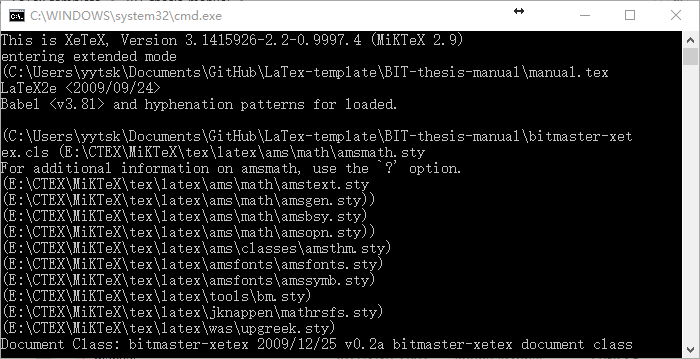
\includegraphics[width=0.8\textwidth]{figures/BIT-thesis-run}
  \caption{BIT-thesis-run.bat脚本运行}
  \label{fig:run}
\end{figure}


\begin{figure}[!htp]
  \centering
  {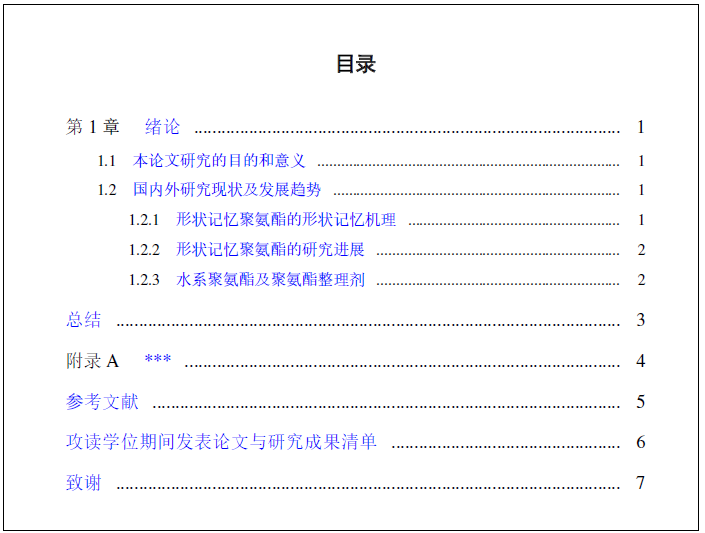
\includegraphics[width=0.8\textwidth]{figures/demo_context}}
  \caption{生成文档demo.pdf的目录}
  \label{fig:demo_context}
\end{figure}

本模板使用~\XeTeX~ 引擎提供的~\XeLaTeX~的命令处理,作用于“主控文档”demo.tex。
由于该模板使用~{{\sc Bib}\TeX}~处理参考文献,构建流程为 \textbf{XeLaTeX$\rightarrow$ BibTeX $\rightarrow$ XeLaTeX$\rightarrow$ XeLaTeX}。完整的处理流程是:

{\color{blue}
\begin{enumerate}
\item[] ~\verb|xelatex -no-pdf --interaction=nonstopmode demo|
\item[] ~\verb|bibtex demo| 
\item[] ~\verb|xelatex -no-pdf --interaction=nonstopmode demo|
\item[] ~\verb|xelatex --interaction=nonstopmode demo|
\end{enumerate}}

运行bibtex的时候会提示一些错误,可能是~{{\sc Bib}\TeX}~对UTF-8支持不充
分,一般不影响最终结果。加入~\verb|--interaction=nonstopmode|~参数是不让错误打断编译过程。
\XeTeX~ 仍存在一些宏包兼容性问题,而这些错误通常不会影响最终的编译结果。

为方便使用,处理过程已经写入BIT-thesis-run.sh(for Linux)和BIT-thesis-run.bat(for Windows)批处理文件中。编写完修改完tex文件后,直接运行对应.sh或者.bat文件即可。

如使用texmaker等编辑器,可使用自定义命令对文档快速构建:

{\color{blue}
\begin{enumerate}
\item[] ~\verb|xelatex -interaction=nonstopmode %.tex ||
\item[] ~\verb|bibtex % || 
\item[] ~\verb|xelatex -interaction=nonstopmode %.tex ||
\item[] ~\verb|xelatex -interaction=nonstopmode %.tex|
\end{enumerate}}


\section{模板说明与Tex介绍}
\label{sec:features}
 
目前网上有两个版本的北理工~\LaTeX~ 模板“2012大眼小蚂蚁版”和“2016汪卫版”,均以上海交通大学的模为基础。本模板在此两个模板的基础上依据《北京理工大学博士、硕士学位论文撰写规范》修改,进一步完善成熟,使得模板能够被北理工硕士博士广泛使用。希望使用者通过本模板的介绍对~\LaTeX~ 有一定了解。

这个模板的中文解决方案是~\XeTeX/\LaTeX~ 。参考
文献建议使用~BibTeX~管理,可以生成符合国标~GBT7714~风格的参考文献列表。
可以直接插入EPS/PDF/JPG/PNG格式的图像。
模板在~Windows~和~Linux~下测试通过,更详细的系统要求请参考
\ref{sec:requirements}。

硕士模板的格式受~bitmater-xetex.cls~和~bitmaster-xetex.cfg~控制,博士模板的格式受~bitdoctor-xetex.cls~和~bitdoctor-xetex.cfg~控制方便模板更新和模板修改。依据《北京理工大学博士、硕士学位论文撰写规范》修改,按照本文档说明使用,即可撰写符合《北京理工大学博士、硕士学位论文撰写规范》的学位论文;
在对外观进行细微调整时,只需要更新这两个文件,不需要对.tex源文件做修改。这也给模板更新带来了
极大方便。\textbf{一般使用者不需要修改这两个文件。}
 
~XeLaTeX~ 对应的XeTeX对中文字体的支持更好,允许用户使用操作系统字体来代替TeX的标准字体。所以本模板使用~XeLaTeX~ 引擎处理中文。要使用这个模板协助你完成研究生学位论文的创作,下面的条件必须满足:

\begin{itemize}
\item  操作系统字体目录中有中文字体(adobe或windows字体均可);
\item  \TeX~系统有~\XeTeX~引擎;
\item  \TeX~系统有~ctex~宏包;
\item  \TeX~系统的fontspec宏包(fontspec.sty)足够新;
\item  你有使用~\LaTeX~的经验。
\end{itemize}

安装完成后,便可对tex进行编写以生成相应论文,也可更具使用习惯使用texmaker、Winedit等其他的编辑器进行编写(推荐使用texmaker)。



